\chapter{Esempio di sessione}%tante immaginine

\begin{figure}[ht!]
	\caption{All'apertura della pagina la mappa si presenta cos\`i. In alto sono presenti i comandi per filtrare i risultati, nella mappa, partendo da sinistra troviamo i pulsanti per lo zoom, quelli per navigare tra i risultati e sulla destra i particolari sul locale selezionato.}
	\centering
		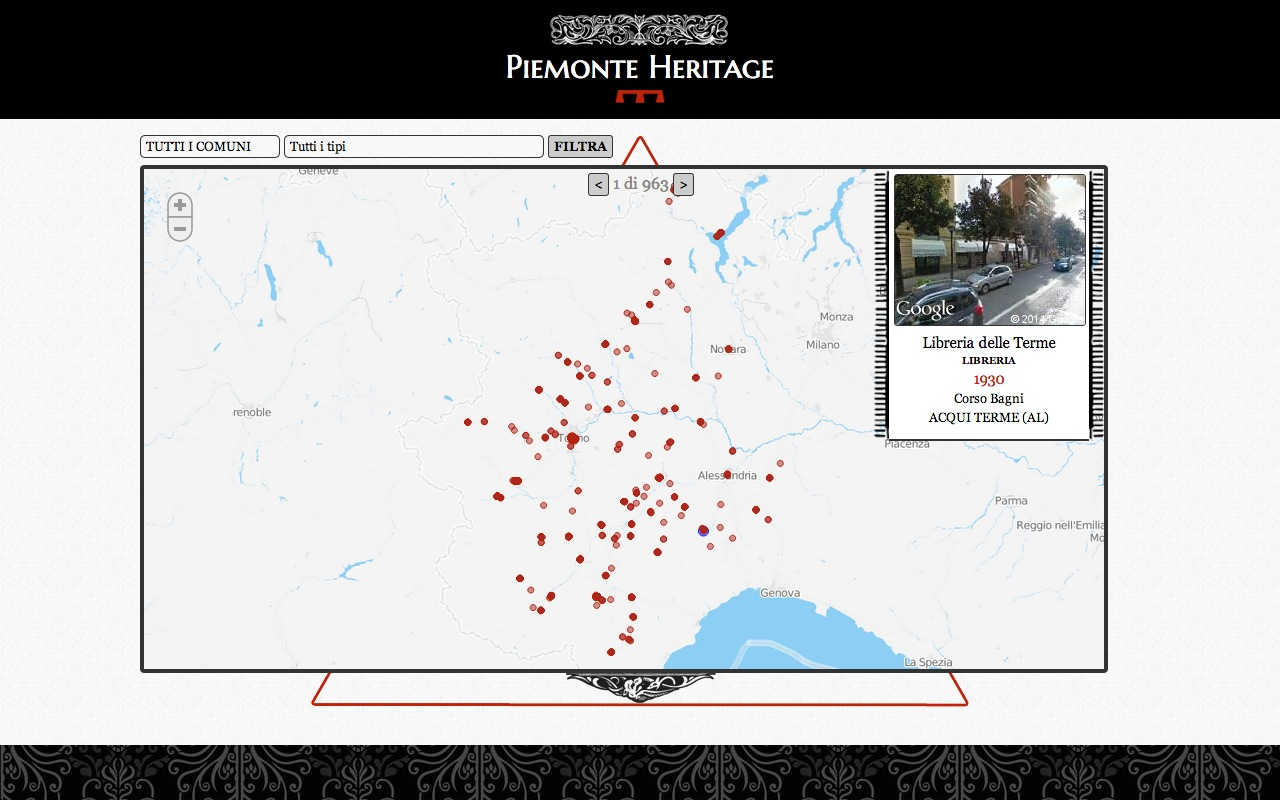
\includegraphics[width=\textwidth]{img/s1.jpg}
\end{figure}

\begin{figure}[ht!]
	\caption{Elenco di tutte le tipologie disponibili}
	\centering
		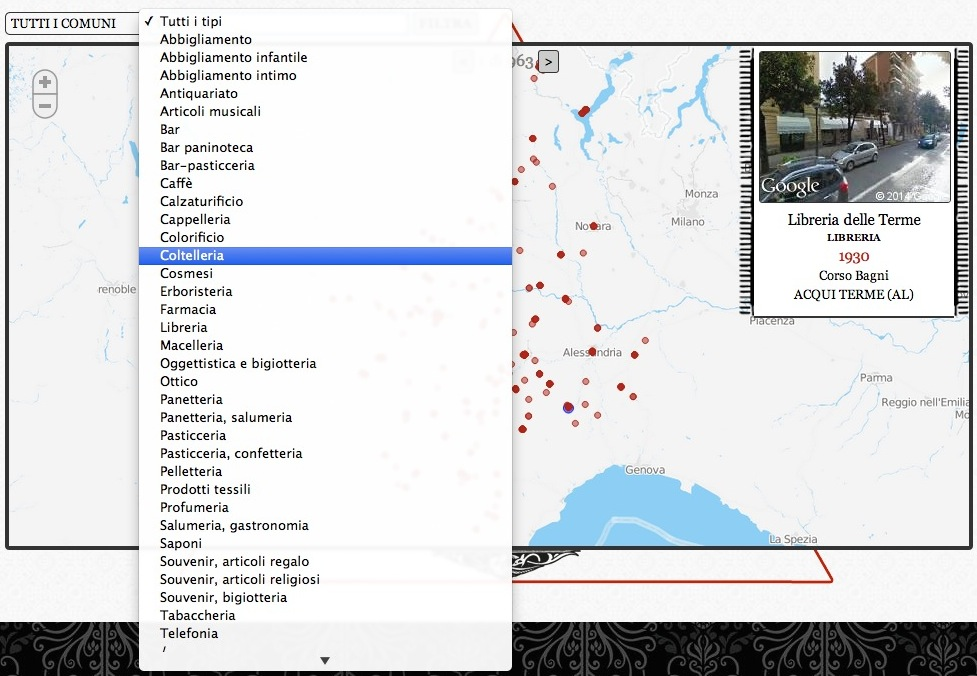
\includegraphics[width=\textwidth]{img/s2.jpg}
\end{figure}

\begin{figure}[ht!]
	\caption{Selezione del comune}
	\centering
		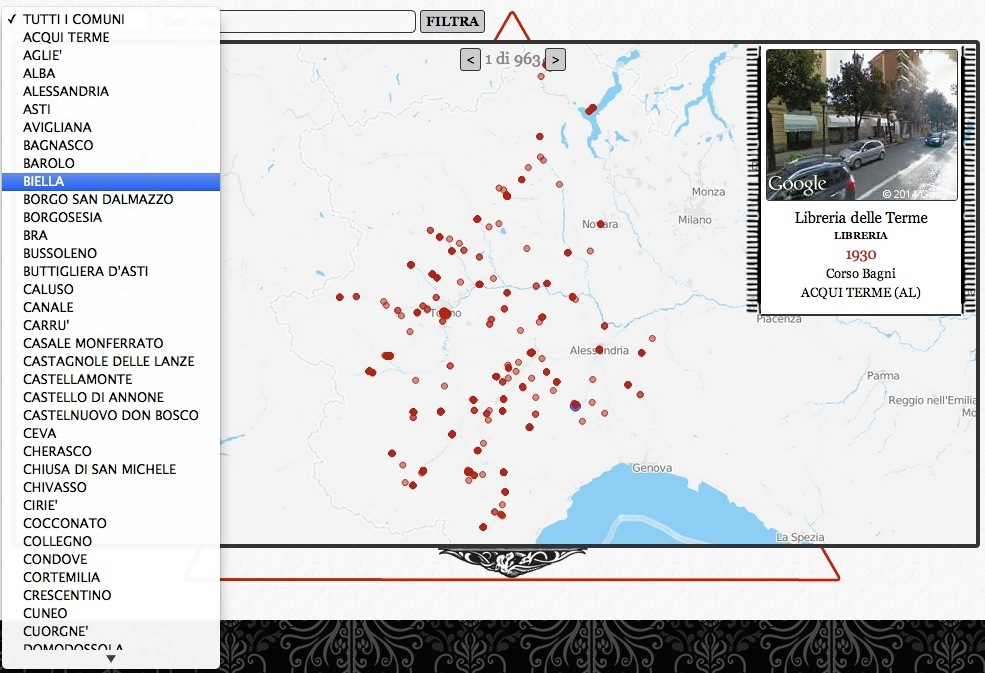
\includegraphics[width=\textwidth]{img/s3.jpg}
\end{figure}

\begin{figure}[ht!]
	\caption{Le tipologie mostrate sono solo quelle presenti nel comune selezionato}
	\centering
		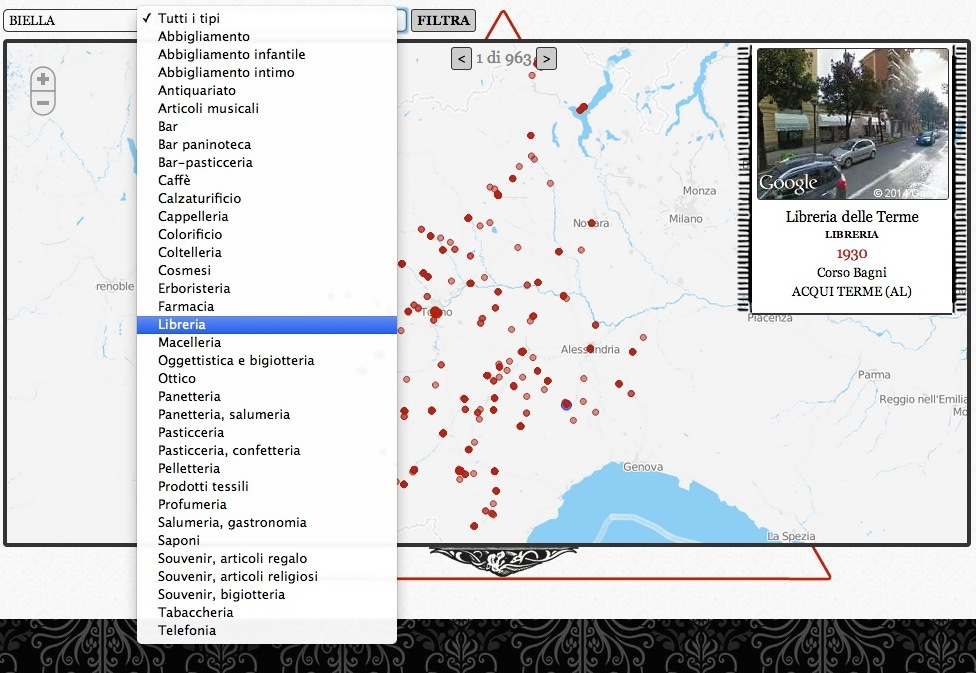
\includegraphics[width=\textwidth]{img/s4.jpg}
\end{figure}

\begin{figure}[ht!]
	\caption{Premendo filtra, vengono mostrati i locali sulla mappa e viene selezionato il primo, mostrando i dati nello specchietto in alto a destra. La mappa mostra solamente i punti filtrati ed effettua un riposizionamento nel modo descritto nel Capitolo \ref{sec:riposizionamento} ed adatta lo zoom in modo da mostrare tutti i punti.}
	\centering
		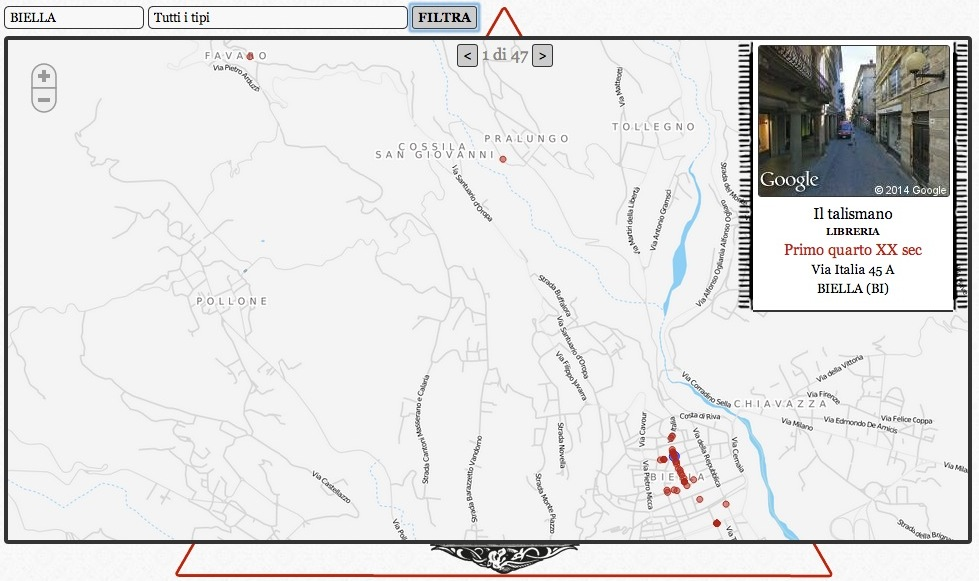
\includegraphics[width=\textwidth]{img/s5.jpg}
\end{figure}

\begin{figure}[ht!]
	\caption{Premendo i pulsanti di navigazione viene selezionato il locale successivo, cambiandone l'indicatore da rosso a blu e centrandolo sulla mappa. I relativi dati inoltre vengono mostrati in alto a destra.}
	\centering
		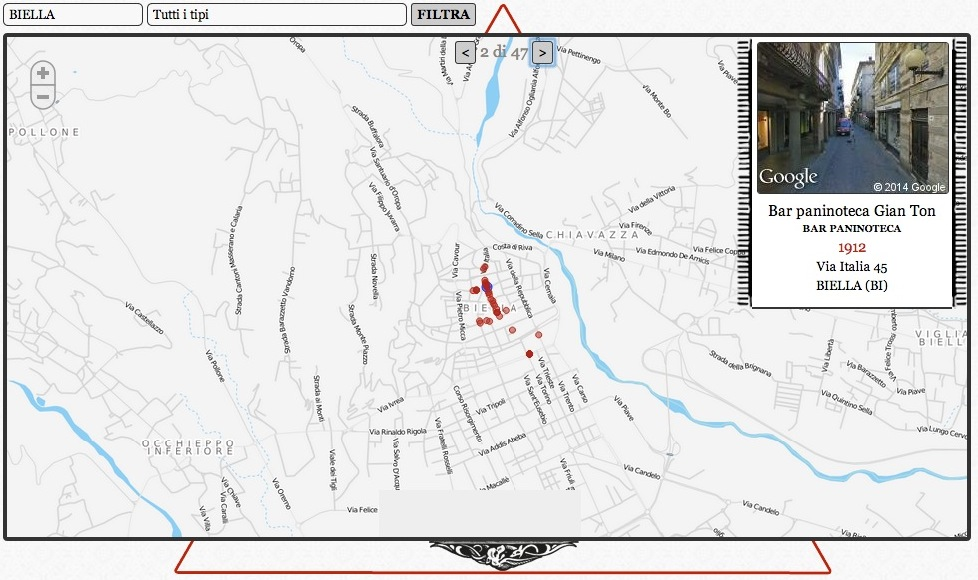
\includegraphics[width=\textwidth]{img/s6.jpg}
\end{figure}

\begin{figure}[ht!]
	\caption{(Valutare se eliminare questa immagine, va solo al punto successivo, come l'immagine precedente.)}
	\centering
		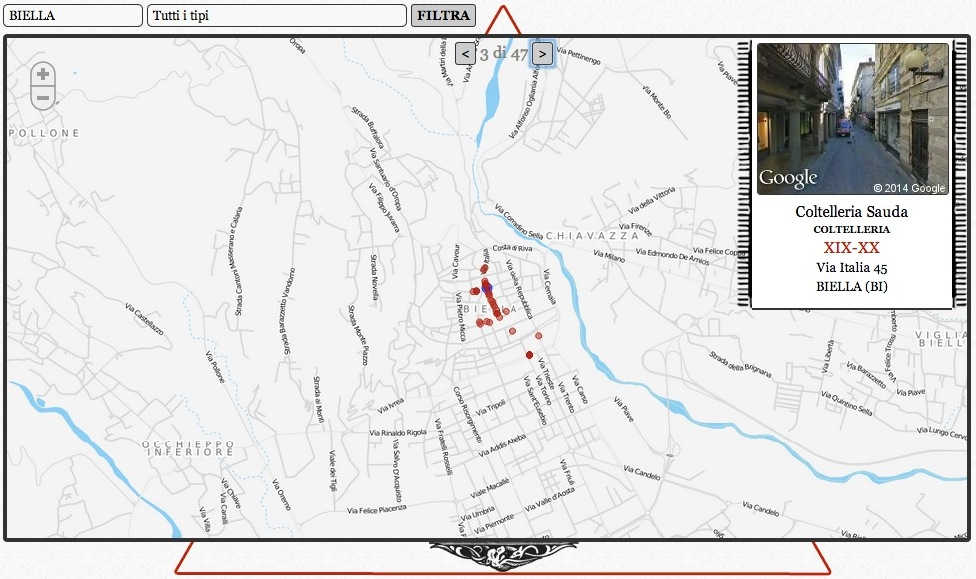
\includegraphics[width=\textwidth]{img/s7.jpg}
\end{figure}

\begin{figure}[ht!]
	\caption{Selezionando una categoria e poi filtra, vengono mostrati solo i relativi punti. In questo caso solo i due bar di Biella presenti nel dataset.}
	\centering
		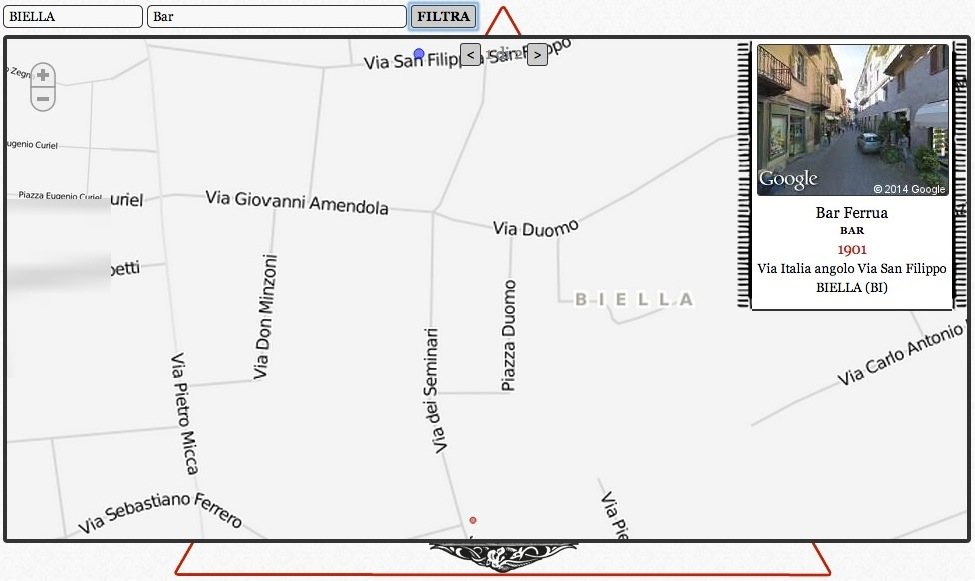
\includegraphics[width=\textwidth]{img/s8.jpg}
\end{figure}

\begin{figure}[ht!]
	\caption{Se lo si desidera, si pu\`o visualizzare tutti i locali dello stesso tipo in tutti i comuni.}
	\centering
		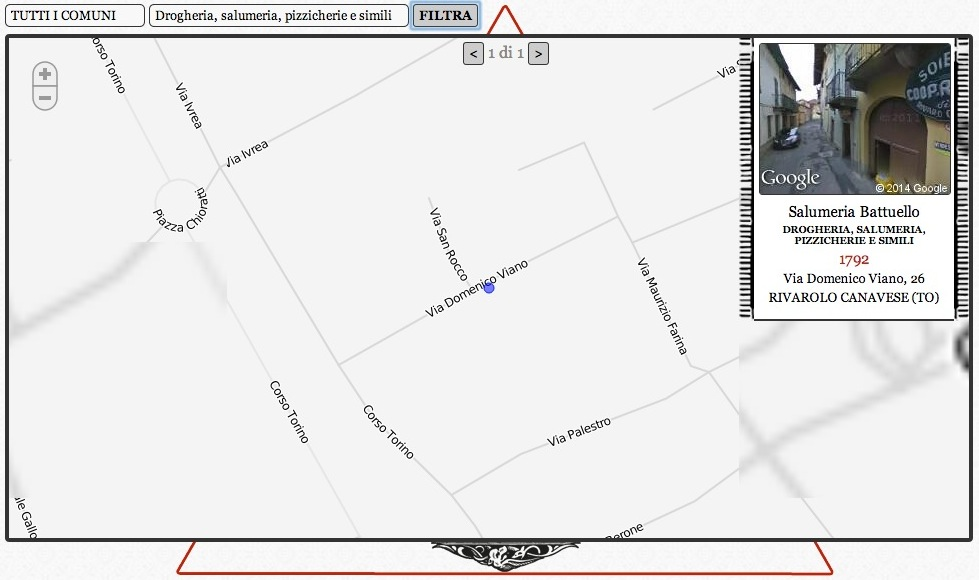
\includegraphics[width=\textwidth]{img/s9.jpg}
\end{figure}

\begin{figure}[ht!]
	\caption{Nel caso in cui, dopo aver selezionato un tipo, si seleziona un comune che non contiene locali di quella categoria, il men\`u a tendina seleziona automaticamente "Tutti i tipi"}
	\centering
		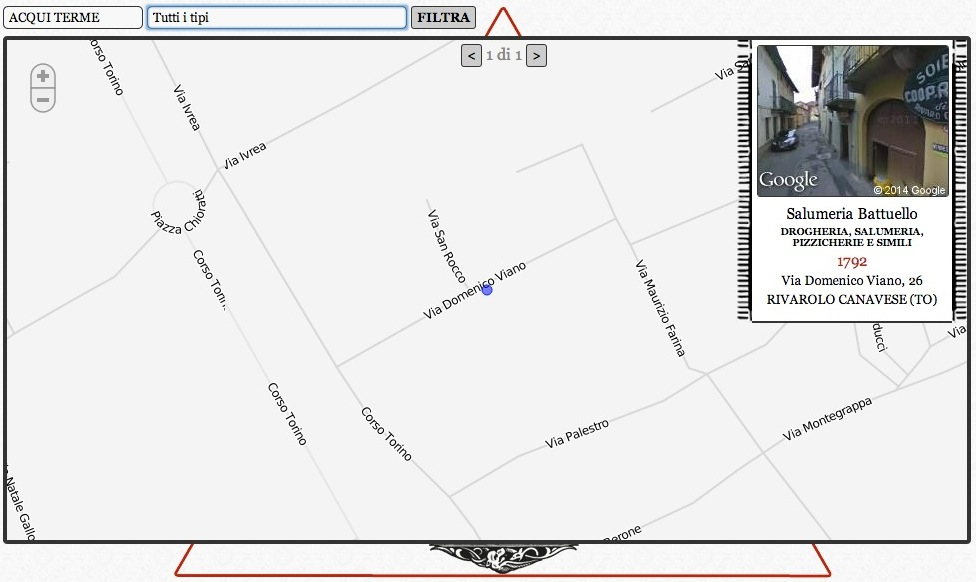
\includegraphics[width=\textwidth]{img/s10.jpg}
\end{figure}

\begin{figure}[ht!]
	\caption{I record non contengono dati esatti: l'ubicazione memorizzata \`e nel comune di Torino, ma le coordinate sono inesatte.}
	\centering
		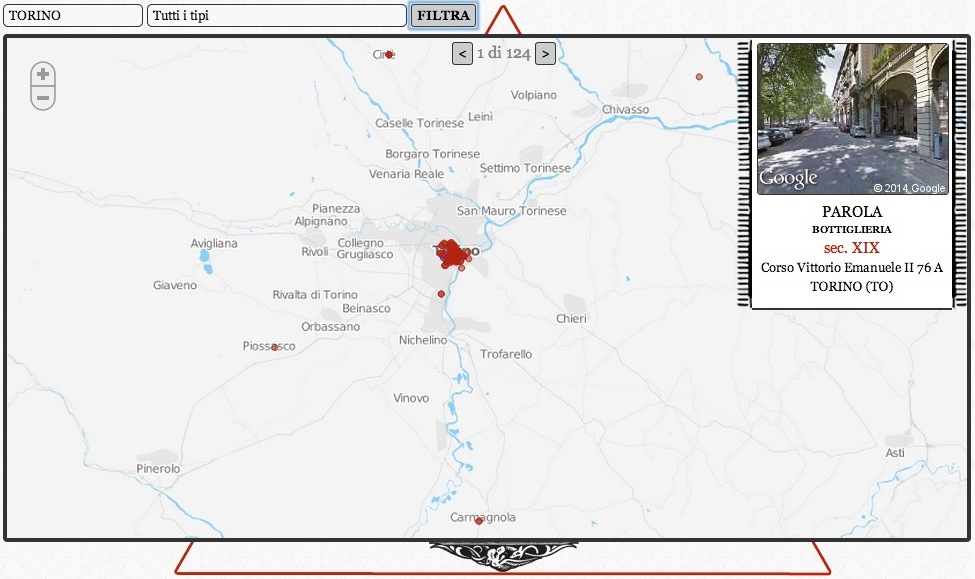
\includegraphics[width=\textwidth]{img/s11.jpg}
\end{figure}

\begin{figure}[ht!]
	\caption{Panoramica dei locali di Torino}
	\centering
		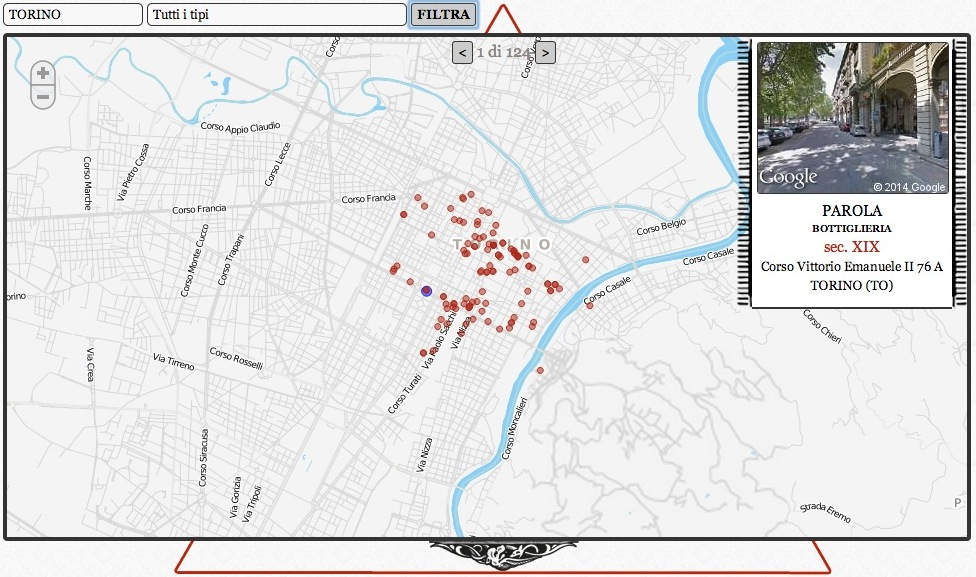
\includegraphics[width=\textwidth]{img/s12.jpg}
\end{figure}

\begin{figure}[ht!]
	\caption{Cliccando su un puntino esso verr\`a selezionato.}
	\centering
		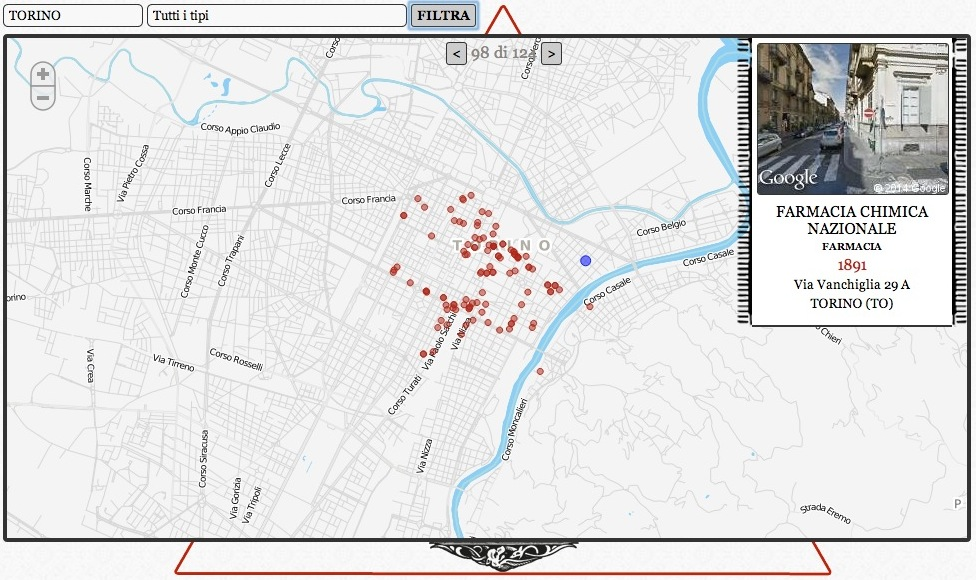
\includegraphics[width=\textwidth]{img/s13.jpg}
\end{figure}ht!